\documentclass[12pt,a4paper]{article}

\usepackage[utf8]{inputenc}
\usepackage[T1]{fontenc}
\usepackage{amsmath,amssymb,amsthm}
\usepackage{mathrsfs}
\usepackage{tikz}
\usetikzlibrary{arrows.meta, positioning, calc}
\usepackage[margin=1in]{geometry}
\usepackage{hyperref}

% Theorem environments
\newtheorem{theorem}{Theorem}[section]
\newtheorem{definition}[theorem]{Definition}
\newtheorem{example}[theorem]{Example}

% Notation shortcuts
\newcommand{\N}{\mathbb{N}}
\newcommand{\R}{\mathbb{R}}
\newcommand{\Nz}{\mathbb{N}_0}
\newcommand{\Rp}{\overline{\R^+}}

\title{On the Inverse Problem of Reaction Kinetics}
\author{V.\ H\'ars \and J.\ T\'oth}
\date{}

\begin{document}

\maketitle

\begin{center}
\textsc{Colloquia Mathematica Societatis J\'anos Bolyai}\\
\textsc{30.\ Qualitative Theory of Differential Equations}\\
\textsc{Szeged (Hungary), 1979.}
\end{center}

\bigskip

%%% ─────────────────────────────────────────────────────
\section{Introduction}

The object most often dealt with in the theory of formal reaction kinetics is the \emph{complex chemical reaction} or \emph{mechanism}.  It means that a vessel is given that contains, say $M$ kinds of different, homogeneously distributed chemical components.  Reactions take place among these components causing the change of the quantities of the components but retaining their spatial homogeneity.  The state of the mechanism is characterized by the vector consisting of the quantities of the components.  Time is considered to be continuous, the state is assumed to change continuously and deterministically.\footnote{Another model, that is very often dealt with, is the continuous time, discrete state stochastic model.  Some of the relations between the properties of these models are treated in our other paper \cite{ErdiTothHars1979} in this volume.}
The change of state is usually described by a system of polynomial differential equations, called \emph{kinetic differential equation}.

We may say that relating a differential equation to a complex chemical reaction and investigating its quantitative and qualitative properties we solve parts of the \emph{direct problem} of chemical reaction kinetics.  On the other side, the \emph{inverse problem} is to determine whether to a given set of qualitative and/or quantitative properties of the kinetic differential equation there exists a complex chemical reaction having the properties given before (\cite{Emanuel1975}, p.~154; \cite{Jacquez1972}, p.~1, 102, 152, 187, 211; \cite{TothErdi1978}, pp.~303--307).  Here it will be called inverse problem only to determine whether to a given system of polynomial differential equations there exists a complex chemical reaction (and if it does, how many) having the given differential equation as its kinetic differential equation.

This step of the inverse problem of reaction kinetics can be formulated \emph{in purely mathematical terms}, using the terminology introduced by Vol'pert \cite{Volpert1972}.  Let us given the transformation that maps the set of oriented bipartite graphs with multiple edges and without loops into the set of polynomial differential equations.  What is the range of this transformation and what is the full inverse of a point of its range?

(There is only a slight difference between the definitions of Vol'pert and those used here and having been developed by Feinberg, Horn and Jackson, see e.g.\ \cite{Feinberg1977}, \cite{TothErdi1978}.)

The solution of the inverse problem has a double significance.  From the \emph{practical} point of view, it is vital to know that a system obtained by model fitting may be considered as a kinetic differential equation or not.  From the \emph{theoretical} point of view, if it is known, that a given differential equation may be considered as a kinetic differential equation then the surprisingly strong theorems on the qualitative behaviour of the kinetic differential equations, such as the zero deficiency theorem or Vol'pert's theorems can be applied.  This second one is the viewpoint of the theoretical biochemist: the man who is seeking for reactions exhibiting exotic behaviour (multistationarity, oscillation, etc.\ \cite{ErdiTothHars1979}.)

In the present paper first we introduce some definitions in order to be able to formulate precisely our problem.  Secondly, we give an (essentially trivial) necessary and sufficient condition for the solvability of the inverse problem and if this condition is fulfilled, we construct the so called canonic mechanism to the differential equation.

Our results outlined here made it possible to determine the structure of mechanisms having a \emph{gradient system} as their kinetic differential equation, i.e.\ having a potential function to the right-hand side of the kinetic differential equation \cite{Toth1979gradient}.


%%% ─────────────────────────────────────────────────────
\section{Notations and Definitions}

For the sake of uniqueness wholly formal definitions will be given below.  Further motivations and clarifications, if necessary, may be found in e.g.\ \cite{Feinberg1977}, \cite{HornJackson1972} and \cite{TothErdi1978}.

Let $M, N \in \N$;\; $S :=\{A(1), \ldots, A(M)\}$.  ($A(m)$ is the symbol of the $m$-th \emph{chemical component};\; $m \in \{1,2,\ldots,M\}$.)  Let us given the set\footnote{$\Nz := \N \cup \{0\}$ is the set of nonnegative integers.} $T := \{C(1), \ldots, C(N)\} \subset \Nz^{\,M}$, the elements of which are called \emph{complexes}, and the set $R \subset T \times T$, the elements of which are called \emph{elementary reactions}.  If $(C(j), C(i)) \in R$, then to write $C(j) \to C(i)$ is preferred and it is said that the \emph{reactant} complex $C(j)$ is transformed into the \emph{product} complex $C(i)$.  It can be assumed that all of the complexes take part in a reaction, i.e.\ for every $n \in \{1,2,\ldots,N\}$ there is an $i \in \{1,2,\ldots,N\}$, such that either $C(i) \to C(n)$ or $C(n) \to C(i)$ is fulfilled.

The natural basis $\mathscr{B}$ of $\R^S$ is formed by the functions $\omega_{A(m)}$ such that
\[
  \omega_{A(m)}(A(i)) = \delta_{im} \qquad (m, i \in \{1,2,\ldots,M\})
\]
(here $\delta_{im}$ is the Kronecker-symbol), accordingly
\[
  \mathscr{B} = \{\omega_{A(m)} ;\; \omega_{A(m)} \in \R^S,\;
  \omega_{A(m)}(A(i)) = \delta_{im},\; m, i \in \{1,2,\ldots,M\}\}.
\]
By these functions all $C(n) \in T$ can be expressed:
\[
  C(n) =: \sum_{m=1}^{M} y^m(n)\, \omega_{A(m)}.
\]
Instead of this last expression one always writes in chemistry and sometimes in linear algebra (\cite{FeinbergHorn1977}, p.~85):
\[
  C(n) = \sum_{m=1}^{M} y^m(n)\, A(m),
\]
and also we shall identify the elements of the natural basis of $\R^S$ with the elements of $S$.

Let the \emph{complex vectors} $y(n)$ be defined as follows:
\[
  y(n) := (y^1(n) \ldots y^M(n))^T \in \Nz^{\,M}
  \qquad (n \in \{1,2,\ldots,N\}),
\]
i.e.\ vectors having the coefficients of the complexes in the natural basis as their coordinates.  (These are called \emph{stoichiometric coefficients} in chemistry.)  Further let
\[
  Y := (\; y(1) \;\ldots\; y(N)\;)
\]
be the \emph{complex matrix}.  (This can be assumed not to have a row of zeros, i.e.\ each chemical component takes part in at least one complex.  Although it may have a column of zeros, this corresponds to the \emph{zero complex}, denoted by $0$.)  By the complex vectors the elementary reaction $C(j) \to C(i)$ will be denoted sometimes by $y(j) \to y(i)$ as well.

Let $V := \R^M$ be the \emph{component space}, and $W := \R^N$ be the \emph{complex space}, and $R$ the function providing the rates, the \emph{kinetics}\footnote{$\R^+$ is the set of positive real numbers, $\Rp$ is the set of nonnegative real numbers.}:
\[
  (\Rp)^M =: V^+ \ni x \mapsto R(x) \in \R^{N \times N}
\]
For each $x \in V^+$ the elements $r_{ij}(x) := (R(x))_{ij}$ of the \emph{rate matrix} $R(x)$ fulfil
\begin{enumerate}
  \item[(i)] $r_{ij}(x) \ge 0 \qquad (i,j \in \{1,2,\ldots,N\})$
  \item[(ii)] $r_{ii}(x) = 0 \qquad (i \in \{1,2,\ldots,N\})$
\end{enumerate}

The reaction $C(j) \to C(i)$ is said to have a rate $r_{ij}(x)$ if the vector of the concentrations of the components is $x$.

\begin{definition}
A \emph{complex chemical reaction} or \emph{mechanism} is an object $\mathsf{M} = \langle M, N, S, T, R, R \rangle$ of elements with the properties described above.
\end{definition}

\begin{definition}
The complex chemical reaction $\mathsf{M}$ is of the \emph{mass action type} if there exists a matrix $K \in \R^{N \times N}$ with nonnegative components and zero main diagonal which gives the rates as follows:
\[
  r_{ij}(x) = k_{ij}\, x^{\,y(j)},
\]
where $k_{ij} := (K)_{ij}$ and the second factor of the right-hand side is defined as usual (\cite{HornJackson1972}, p.~90):
\[
  x^{\,y(j)} := \prod_{m=1}^{M} x_m^{y^m(j)}.
\]
\end{definition}

\begin{definition}
The (continuous time, continuous state) \emph{deterministic model} or \emph{kinetic differential equation} of the mechanism is the following explicit first order differential equation:
\[
  \dot{x}(t) = Y\bigl[\, R(x(t)) - R(x(t))^T\,\bigr] \mathbf{1}_N
\]
\[
  (D_x \subset \R^+;\; R_x \subset \R^M;\; t \in D_x \;;\; \mathbf{1}_N = (1,1,\ldots,1)^T \in \R^N).
\]
\end{definition}

It is easy to show that the kinetic differential equation of a mechanism of the mass action type is of the following form:
\begin{equation}\label{eq:kde}
  \dot{x}(t) = Y\bigl[\,K - \operatorname{dg} K^T \mathbf{1}_N\,\bigr]\, x(t)^Y
  = \sum_{p=1}^{N} \sum_{q=1}^{N} k(p,q)\bigl(\,y(p) - y(q)\,\bigr)\, x(t)^{\,y(q)}
\end{equation}
$(t \in D_x)$, where
\[
  \R^N \ni z \mapsto \operatorname{dg} z :=
  \begin{pmatrix}
    z_1 & 0 & \cdots & 0 \\
    0 & z_2 &        & 0 \\
      &     & \ddots &   \\
    0 & \cdots &      & z_N
  \end{pmatrix}
  \in \R^{N \times N}
\]
if $z = (z_1, z_2, \ldots, z_N)^T$;\; and
\[
  x(t)^Y := (\; x(t)^{\,y(1)} \;\ldots\; x(t)^{\,y(N)}\;)^T.
\]

In this paper \emph{only mechanisms of the mass action type} will be dealt with.  These are determined by $M$, $N$, $S$, $T$, $R$ and $K$, therefore they will be denoted -- with a bit of inexactness -- by $\langle M, N, S, T, R, K \rangle$.


%%% ─────────────────────────────────────────────────────
\section{Solution of the Inverse Problem}

Here we state a property of the kinetic differential equation \eqref{eq:kde} that will prove to be characteristic.  In other words, a necessary condition for the solvability of the inverse problem will be given, then it will be proved that this condition is sufficient as well.

Difficult it may be to formulate, the condition is self-evident.

\begin{definition}\label{def:polynomial}
Let $M \in \N$.  The function $P \colon \R^M \to \R^M$ is a \emph{polynomial of $M$ variables}, if for each $m, m' \in \{1,2,\ldots,M\}$ and for each $x_1, x_2, \ldots, x_{m-1}, x_{m+1}, \ldots, x_M \in \R$ the function
\[
  \mathrm{pr}_{m'} \circ P(x_1, x_2, \ldots, x_{m-1}, \cdot, x_{m+1}, \ldots, x_M) \colon \R \to \R
\]
is a polynomial.  (Here $\circ$ is the sign of composition of functions;\; $\mathrm{pr}_{m'} \colon \R^M \to \R$ is the projection on the $m'$th coordinate.)  This means that there exist parameters
\begin{align}\label{eq:params}
  & I_1, I_2, \ldots, I_M;\; J_1, J_2, \ldots, J_M \in \Nz; \notag \\
  & y_i^m \in \Nz^M,\; \psi_i^m \in \R^+ \quad
    (m \in \{1,2,\ldots,M\},\; i \in \{1,2,\ldots,I_m\}) \notag \\
  & z_i^m \in \Nz^M,\; \nu_i^m \in \R^+ \quad
    (m \in \{1,2,\ldots,M\},\; i \in \{1,2,\ldots,J_m\})
\end{align}
such that for each $m \in \{1,2,\ldots,M\}$ the vectors $y_1^m, \ldots, y_{I_m}^m$ and $z_1^m, \ldots, z_{J_m}^m$ are pairwise different and that for each $x \in \R^M$ and $m \in \{1,2,\ldots,M\}$
\[
  \mathrm{pr}_m(P(x)) = \sum_{i=1}^{I_m} \psi_i^m\, x^{\,y_i^m}
  - \sum_{i=1}^{J_m} \nu_i^m\, x^{\,z_i^m}.
\]
(It is understood that if e.g.\ $I_m = 0$ then there do not exist $y_i^m$ and $\psi_i^m$ and the first sum is zero.)
\end{definition}

\begin{theorem}\label{thm:necessary}
The kinetic differential equation of the mechanism $\mathsf{M} = \langle M, N, S, T, R, K \rangle$ is of the form
\[
  \dot{x} = P \circ x\,,
\]
where $P \colon \R^M \to \R^M$ is a polynomial of $M$ variables, for the parameters of which
\[
  \mathrm{pr}_m(z_i^m) > 0
\]
holds, whenever $J_m > 0$, for each $i \in \{1,2,\ldots,J_m\}$.
\end{theorem}

\begin{proof}
Starting from the form
\[
  \dot{x}(t) = \sum_{p=1}^{N} \sum_{q=1}^{N}
  k(p,q)\bigl(\,y(p) - y(q)\,\bigr)\, x(t)^{\,y(q)}
  \qquad (t \in D_x)
\]
of the kinetic differential equation we can see that the $m$-th coordinate of the right hand side of the equation is
\[
  \sum_{p=1}^{N} \sum_{q=1}^{N} k(p,q)\, y^m(p)\, x(t)^{\,y(q)}
  - \sum_{q=1}^{N} y^m(q)\, x(t)^{\,y(q)} \times \sum_{p=1}^{N} k(p,q).
\]
Here the coefficient of $x(t)^{\,y(q)}$ in the second term differs from zero if and only if $\sum_{p=1}^{N} k(p,q) > 0$ and $y^m(q) > 0$ holds at the same time.
\end{proof}

Now we show that all the differential equations having the peculiar property of kinetic differential equations expressed in Theorem~\ref{thm:necessary} -- that may be called \emph{the lack of negative cross-effects} -- may be considered as kinetic differential equations.

\begin{theorem}\label{thm:sufficient}
Let $M \in \N$, $P \colon \R^M \to \R^M$ be a polynomial of $M$ variables and let us suppose that $P$ fulfils the necessary condition imposed upon the right-hand side of a kinetic differential equation in Theorem~\ref{thm:necessary}.  Then there exists a mechanism $\mathsf{M} = \langle M, N, S, T, R, K \rangle$ having
\begin{equation}\label{eq:kde2}
  \dot{x} = P \circ x
\end{equation}
as its deterministic model.
\end{theorem}

The \textsc{proof} is constructive: a mechanism will be provided having \eqref{eq:kde2} as its deterministic model.  This construction leads to a unique mechanism, called \emph{canonic mechanism} attached to the differential equation \eqref{eq:kde2}.  Obviously, there are many other mechanisms having the same kinetic differential equation.

Let the elements of the set of the complex vectors be defined (some of them twice or more) as follows:
\[
  y_i^m,\; y_i^m + e_m, \quad m \in \{1,2,\ldots,M\},\;
  i \in \{1,\ldots,I_m\};
\]
\[
  z_i^m,\; z_i^m - e_m, \quad m \in \{1,2,\ldots,M\},\;
  i \in \{1,\ldots,J_m\},
\]
where $e_m \in \R^M$ is the $m$-th vector of the natural basis of $\R^M$.

According to the assumption of lack of negative cross-effects all of the coordinates of the vector $z_i^m - e_m$ are nonnegative.  Let the reactions be
\begin{equation}\label{eq:canonic_reactions}
  y_i^m \to y_i^m + e_m, \qquad z_i^m \to z_i^m - e_m
\end{equation}
with reaction rate constants $\psi_i^m$ and $\nu_i^m$, respectively (for all of the values of the indices).  It can be easily verified that the kinetic differential equation of this mechanism is \eqref{eq:kde2}, where the parameters of the polynomial $P$ are those given under \eqref{eq:params}.

\begin{example}\label{ex:canonic}
Let us given the differential equation
\begin{equation}\label{eq:example}
\begin{aligned}
  \dot{x} &= -2\alpha\, x^2 v + 2\gamma\, z^4 \\
  \dot{y} &= 3\alpha\, x^2 v - 3\beta\, y^3 v^2 \\
  \dot{z} &= 4\beta\, y^3 v^2 - 4\gamma\, z^4 \\
  \dot{v} &= \alpha\, x^2 v - 2\beta\, y^3 v^2 + \gamma\, z^4.
\end{aligned}
\end{equation}

The canonic mechanism attached to \eqref{eq:example} is:

\bigskip
\begin{center}
\begin{tikzpicture}[
  node distance=1.8cm and 2.2cm,
  every node/.style={font=\small},
  >=Stealth,
  arrow/.style={->, thick}
]
% Left tree
\node (top1) {$2X+V$};
\node [below left=1.2cm and 1.5cm of top1] (bl1) {$X+V$};
\node [below right=1.2cm and 0cm of top1] (br1) {$2X+2V$};
\node [below=2.4cm of top1] (bot1) {$2X+Y+V$};

\draw[arrow] (top1) -- node[above left] {$2\alpha$} (bl1);
\draw[arrow] (top1) -- node[right] {$\alpha$} (br1);
\draw[arrow] (top1) -- node[below left] {$3\alpha$} (bot1);

% Middle tree
\node [right=4cm of top1] (top2) {$4Z$};
\node [below left=1.2cm and 0.5cm of top2] (bl2) {$X+4Z$};
\node [below right=1.2cm and 0.5cm of top2] (br2) {$4Z+V$};
\node [below=2.4cm of top2] (bot2) {$3Z$};

\draw[arrow] (top2) -- node[above left] {$2\gamma$} (bl2);
\draw[arrow] (top2) -- node[above right] {$\gamma$} (br2);
\draw[arrow] (top2) -- node[right] {$4\gamma$} (bot2);

% Bottom tree
\node [below=4.5cm of $(top1)!0.5!(top2)$] (top3) {$3Y+2V$};
\node [below left=1.2cm and 1cm of top3] (bl3) {$2Y+2V$};
\node [below right=1.2cm and 1cm of top3] (br3) {$3Y+V$};
\node [below=2.4cm of top3] (bot3) {$3Y+Z+2V$};

\draw[arrow] (top3) -- node[above left] {$3\beta$} (bl3);
\draw[arrow] (top3) -- node[above right] {$2\beta$} (br3);
\draw[arrow] (top3) -- node[right] {$4\beta$} (bot3);
\end{tikzpicture}
\end{center}

\bigskip

On the other hand, the kinetic differential equation of the mechanism
\begin{equation}\label{eq:simple_mechanism}
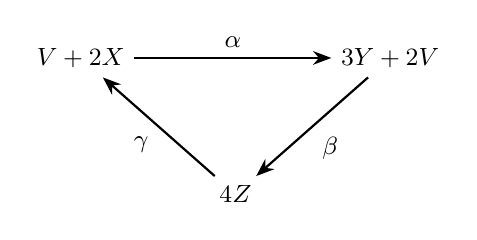
\begin{tikzpicture}[baseline=(current bounding box.center),
  node distance=1.5cm,
  every node/.style={font=\small},
  >=Stealth,
  arrow/.style={->, thick}
]
\node (vx) {$V+2X$};
\node [right=2.5cm of vx] (yv) {$3Y+2V$};
\node [below=1.5cm of $(vx)!0.5!(yv)$] (z) {$4Z$};

\draw[arrow] (vx) -- node[above] {$\alpha$} (yv);
\draw[arrow] (yv) -- node[below right] {$\beta$} (z);
\draw[arrow] (z) -- node[below left] {$\gamma$} (vx);
\end{tikzpicture}
\end{equation}
is also \eqref{eq:example}.

This example shows that the canonic mechanism is not the simplest, neither it is minimal in any sense.  Its only advantage is that it can be constructed very quickly and algorithmically.
\end{example}

Some of the questions arising here -- and outnumbering those answered here -- are as follows:
\begin{enumerate}
  \item For the sake of easy handling we may look for a mechanism with the minimal number of complexes, elementary reactions, linkage classes etc.\ What kind of reasonable assumptions makes this mechanism unique?

  \item We may look for a mechanism in a class of mechanisms with a given -- chemically relevant -- property.  Such a property may be conservativity, (weak) reversibility, zero deficiency or just structural stability as well.  When will a mechanism having the prescribed differential equation as its deterministic model be found within the given class of mechanisms, will it be unique, or, if not, how much not?

  \item A similar, but more complicated problem will be obtained, if only an ``essential'' part of the differential equation is considered.  A problem of this kind has been solved in \cite{TothHars1979compartment} for a special case of first order reactions -- for \emph{compartment systems}.
\end{enumerate}


%%% ─────────────────────────────────────────────────────
\subsection*{Acknowledgements}

This work has been supported in part by the Scientific Research Council, Ministry of Health, Hungary (I-08-0201-03-0/FS).  We are very grateful to our colleagues for their comments.


%%% ─────────────────────────────────────────────────────
\begin{thebibliography}{14}

\bibitem{Emanuel1975}
N.~Emanuel -- D.~Knorre, \emph{Cin\'etique chimique}, ``Mir'', Moscow, 1975.

\bibitem{ErdiTothHars1979}
P.~\'Erdi -- J.~T\'oth -- V.~H\'ars, Exotic phenomena in chemical systems, \emph{Qualitative Theory of Differential Equations}, Szeged, 1979, Colloq.\ Math.\ Soc.\ J\'anos Bolyai~30.

\bibitem{Feinberg1972}
M.~Feinberg, Complex balancing in general kinetic systems, \emph{Arch.\ Rational Mech.\ Anal.}, 49(1972), 187--194.

\bibitem{Feinberg1977}
M.~Feinberg, Mathematical aspects of mass action kinetics, in \emph{Chemical Reactor Theory: A Review} (Eds.\ N.~Amundson and L.~Lapidus) Prentice Hall, Englewood Cliffs, 1977, 1--78.

\bibitem{FeinbergHorn1977}
M.~Feinberg -- F.J.M.~Horn, Chemical mechanism structure and the coincidence of the stoichiometric and kinetic subspaces, \emph{Arch.\ Rational Mech.\ Anal.}, 66(1977), 83--97.

\bibitem{Horn1972}
F.~Horn, Necessary and sufficient conditions for complex balancing in chemical kinetics, \emph{Arch.\ Rational Mech.\ Anal.}, 49(1972), 172--186.

\bibitem{HornJackson1972}
F.~Horn -- R.~Jackson, General mass action kinetics, \emph{Arch.\ Rational Mech.\ Anal.}, 47(1972), 81--116.

\bibitem{Jacquez1972}
J.A.~Jacquez, \emph{Compartmental analysis in biology and medicine}, Elsevier Publishing Co., Amsterdam--London--New York, 1972.

\bibitem{KanyarToth1976}
B.~Kany\'ar -- J.~T\'oth, Fitting of a system of linear differential equations by gradient method (in Hungarian), \emph{Alk.\ Mat.\ Lapok} 2(1976), 259--268.

\bibitem{Lovasz1979}
L.~Lov\'asz, \emph{Combinatorial problems and exercises}, Akad\'emiai Kiad\'o, Budapest and North-Holland Publishing Company, Amsterdam--New York--Oxford, 1979.

\bibitem{Toth1979gradient}
J.~T\'oth, Gradient systems are cross-catalytic, \emph{React.\ Kinet.\ Catal.\ Lett.}, 12(1979), 253--257.

\bibitem{TothErdi1978}
J.~T\'oth -- P.~\'Erdi, Models, problems and applications of formal reaction kinetics, \emph{A k\'emia \'ujabb eredm\'enyei} (in Hungarian), 41(1978), 226--352.

\bibitem{TothHars1979compartment}
J.~T\'oth -- V.~H\'ars, On the inverse problem of compartment systems (in Hungarian), \emph{Alk.\ Mat.\ Lapok}, 5(1979), 49--61.

\bibitem{Volpert1972}
A.I.~Vol'pert, Differential equations on graphs (in Russian), \emph{Mat.\ sbornik}, 88(1972), 578--588.

\end{thebibliography}

\bigskip
\noindent
V.~H\'ars -- J.~T\'oth\\
Computing Group\\
Semmelweis University Medical School\\
Kulich Gyula t\'er~5, H-1089 Budapest, Hungary

\end{document}
